\section{Rechnung an einem Konkreten Beispiels}

\subsection{Brechungsgesetz von Snellius}
\cite{Wikipedia}Aus dem Fermatschen Prinzip lässt sich das Brechungsgesetz von Snellius herleiten.
Das Licht legt den Weg vom Startpunkt $P_0$ über den Brechungspunkt $P_1$ 
nach dem Endpunkt $P_2$ zurück. Dadurch kann die zurückgelegte Zeit berechnet werden.

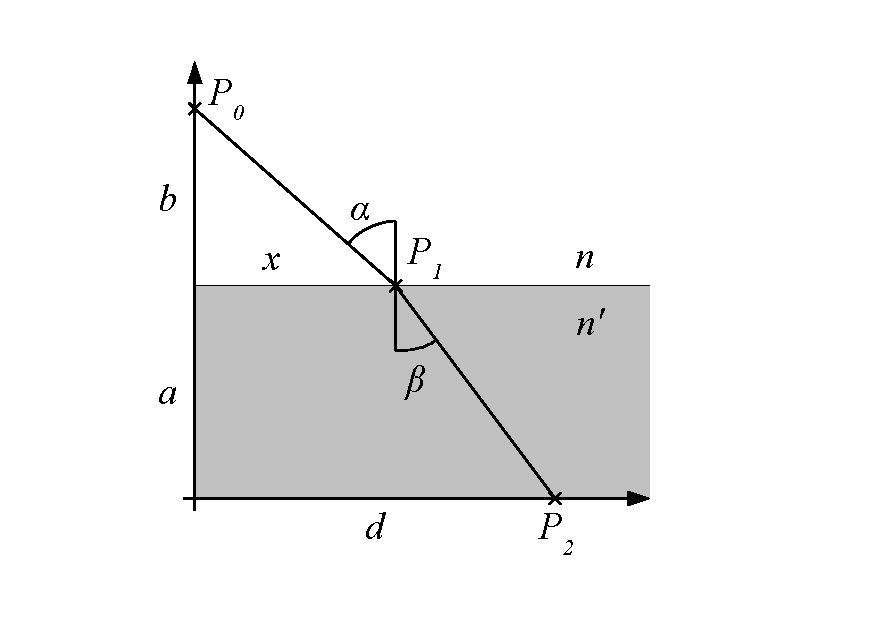
\includegraphics{./picture/Brechung.pdf}



\[
t(x) =
t_1 + t_2 =
\frac{s_1}{c_1} + \frac{s_2}{c_2} =
\frac{|P_1 - P_0|}{c_1} + \frac{|P_2 - P_1|}{c_2} =
\frac{\sqrt{a^2 + x^2}}{c_1} + \frac{\sqrt{(d-x)^2 + b^2}}{c_2}
\]

Leiten wir diese Funktion nun nach $x$ ab, finden wir eine Extremalstelle von $t$.

\[
0 = 
\frac{dt}{dx} =
\frac{2 \cdot x}{2 \cdot c_1 \cdot \sqrt{a^2 + x^2}} + 
\frac{-2 \cdot (d-x)}{2 \cdot c_2 \cdot \sqrt{(d-x)^2 + b^2}} =
\frac{x}{c_1 \cdot \sqrt{a^2 + x^2}} - 
\frac{(d-x)}{c_2 \cdot \sqrt{(d-x)^2 + b^2}}
\]

Aus dem Bild kann man schön sehen, dass $x = \sin(\alpha) \cdot \sqrt{a^2 + x^2}$
und $d-x = \sin(\beta) \cdot \sqrt{(d -x)^2 + b^2}$

\[
0 = 
\frac{\sin(\alpha)}{c_1} - \frac{\sin(\beta)}{c_2} \Leftrightarrow
\frac{c_2}{c_1} = \frac{\sin(\beta)}{\sin(\alpha)}
\]

%Diese Funktion bis jetzt ist ja schön und gut, 
%jedoch konnte noch nicht nachgewiesen werden, 
%dass die Extremalstelle auch wirklich ein Minimum ist. 
%Deshalb müssen wir nun noch die zweite Ableitung berechnen.

%\[
%0 > 
%\frac{dt^2}{d^2x} \left(\frac{\sqrt{a^2 + x^2}}{c_1} + 
%\frac{\sqrt{(d-x)^2 + b^2}}{c_2}\right) =
%\frac{dt}{dx} \left(\frac{x}{c_1 \cdot \sqrt{a^2 + x^2}} - 
%\frac{(d-x)}{c_2 \cdot \sqrt{(d-x)^2 + b^2}} \right) = \phantom a
%\]
%\[
%- \frac{x^2}{c_1 \cdot \sqrt{(a^2 + x^2)}^{3}}
%+ \frac{1}{c_1 \cdot \sqrt{a^2 + x^2}}
%+ \frac{(d-x)\cdot(x-d)}{c_2 \cdot \sqrt{(b^2 + (d - x)^2)}^{3}}
%+ \frac{1}{c_2 \cdot \sqrt{b^2 + (d-x)^2}} = \phantom a
%\]
%\[
%\frac{a^2}{c_1 \cdot \sqrt{(a^2 + x^2)}^{3}}
%+ \frac{b^2}{c_2 \cdot \sqrt{(b^2 + (d - x)^2)}^{3}} = \phantom a
%\]

\subsection{Reflexionsgesetz}
\cite{Wikipedia}Genau gleich wie aus dem Fermatschen Prinzip das Brechungsgesetz herleiten liess, 
lässt sich daraus auch das Reflexionsgesetz ableiten.
Das Licht legt den Weg vom Startpunkt $P_0$ über den Spiegelpunkt $P_1$ 
nach dem Endpunkt $P_2$ zurück. Dadurch kann die zurückgelegte Zeit berechnet werden.

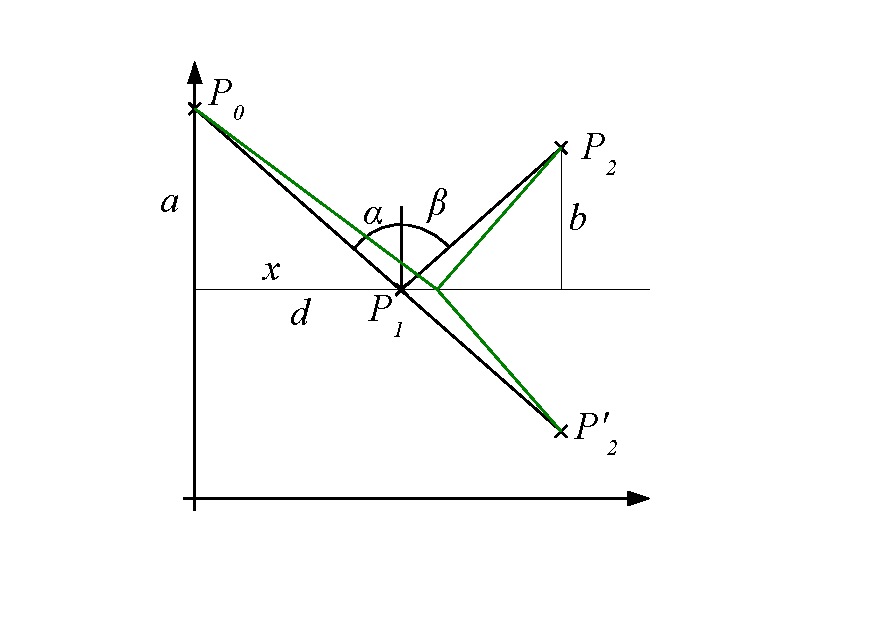
\includegraphics{./picture/Spiegelung.pdf}


\[
t(x) =
t_1 + t_2 =
\frac{s_1 + s_2}{c} =
\frac{|P_1 - P_0| + |P_2 - P_1|}{c} =
\frac{\sqrt{a^2 + x^2} + \sqrt{(d-x)^2 + b^2}}{c}
\]

Leiten wir diese Funktion nun nach $x$ ab, finden wir eine Extremalstelle von $t$.

\[
0 = 
\frac{dt}{dx} =
\frac{1}{c} \cdot
\frac{2 \cdot x}{2 \cdot \sqrt{a^2 + x^2}} + 
\frac{-2 \cdot (d-x)}{2 \cdot \sqrt{(d-x)^2 + b^2}} =
\frac{x}{ \sqrt{a^2 + x^2}} - 
\frac{(d-x)}{ \sqrt{(d-x)^2 + b^2}}
\]

Aus dem Bild kann man schön sehen, dass $x = \sin(\alpha) \cdot \sqrt{a^2 + x^2}$
und $d-x = \sin(\beta) \cdot \sqrt{(d -x)^2 + b^2}$

\[
0 = \sin(\alpha) - \sin(\beta) \Leftrightarrow
sin(\beta) = \sin(\alpha) \Leftrightarrow
\beta = \alpha
\]

Im Bild oben kann man schön sehen, dass Linie des Startpunktes bis zum 
gespiegelten Endpunkt eine Gerade ist. Eine Gerade ist immer die Funktion mit dem kürzestem Weg.

%Diese Funktion bis jetzt ist ja schön und gut, 
%jedoch konnte noch nicht nachgewiesen werden, 
%dass die Extremalstelle auch wirklich ein Minimum ist. 
%Deshalb müssen wir nun noch die zweite Ableitung berechnen.

%\[
%0 > 
%\frac{dt^2}{d^2x} \left(\frac{\sqrt{a^2 + x^2}}{c_1} + 
%\frac{\sqrt{(d-x)^2 + b^2}}{c_2}\right) =
%\frac{dt}{dx} \left(\frac{x}{c_1 \cdot \sqrt{a^2 + x^2}} - 
%\frac{(d-x)}{c_2 \cdot \sqrt{(d-x)^2 + b^2}} \right) = \phantom a
%\]
%\[
%- \frac{x^2}{c_1 \cdot \sqrt{(a^2 + x^2)}^{3}}
%+ \frac{1}{c_1 \cdot \sqrt{a^2 + x^2}}
%+ \frac{(d-x)\cdot(x-d)}{c_2 \cdot \sqrt{(b^2 + (d - x)^2)}^{3}}
%+ \frac{1}{c_2 \cdot \sqrt{b^2 + (d-x)^2}} = \phantom a
%\]
%\[
%\frac{a^2}{c_1 \cdot \sqrt{(a^2 + x^2)}^{3}}
%+ \frac{b^2}{c_2 \cdot \sqrt{(b^2 + (d - x)^2)}^{3}} = \phantom a
%\]

\subsection{Fata Morgana}

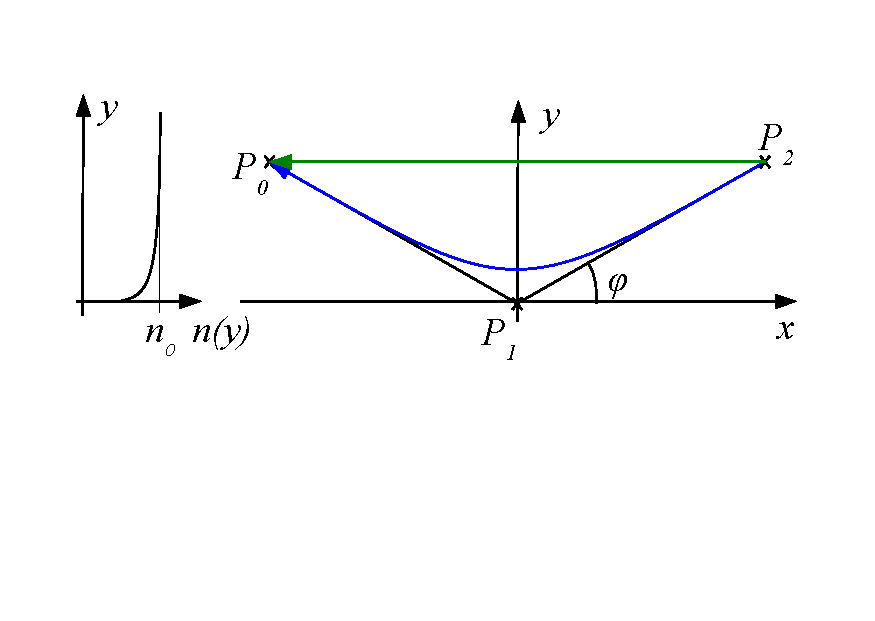
\includegraphics{./picture/FataMorgana.pdf}

Wir nehmen an, wir hätten eine Fata Morgana. 
Dabei hat der Brechungsindex folgende Funktion in Abhängigkeit von $y$ 
(Der Höhe über dem Boden).

\[
n = n_0 (1 - \varepsilon e^{- \alpha y})
\]

Dabei ist der Effekt relativ klein, da $\epsilon << 1$ ist und 
die Skalenlänge $\alpha$ in der Grössenordnung von $\alpha = 1 \cdot m^{-1}$ ist.
Zusätzlich können wir für die Skalierung der x-Richtung die konstante $C$ einführen,
welche wie folgt definiert ist:

\[
C = n \frac{dx}{ds}
\]

Nun betrachten wir die Strahlengleichung komponentenweise für $r = (y(x), x)$ 
und können daraus die Strahlengleichung aufschreiben und vereinfachen.

\[
\frac{d}{ds} \left ( n \frac{dy}{ds} \right ) =
\frac{d}{dx} \left ( n \frac{dy}{dx} \frac{dx}{ds} \right ) \frac{dx}{ds} =
\frac{d}{dx} \left ( C \frac{dy}{dx} \right ) \frac{C}{n} =
\frac{\partial n(y)}{\partial y}
\]

Da die Konstante $C$ nur die x-Achse skaliert, wählen wir diese mit dem Wert $1$.
Wegen $2 n \partial n / \partial y = \partial n^2 / \partial y$ und 
$n^2 \simeq n_0^2(1 - 2 \varepsilon e^{-\alpha y})$ erhalten wir folgende Gleichung.

\[
\frac{d^2 y(x)}{dx^2} =
\frac{1}{2} \frac{\partial}{\partial y} n^2(y) =
n_0^2 \varepsilon \alpha e^{-\alpha y}
\]

Diese Gleichung können wir mit elementaren Methoden gelöst werden. 
Zudem führen wir den Steigungswinkel $\varphi$ ein und schreiben mit 
$\kappa = (\frac{\alpha}{2}) \tan(\varphi)$ können wir die Gleichung einfacher schreiben.

\[
y =
y_0 + \frac{1}{\alpha} ln(\cosh^2(\kappa(x - x_0))) \xrightarrow{\kappa (x - x_0 ) >> 1}
y =
y_0 + \frac{2 \kappa}{\alpha} (x - x_0)
\]

In grossen Abständen zum Spiegelpunkt $x_0$ ist die Ausbreitung des Lichtes geradlinig.
Der Beobachter sieht, wie erwarted zwei Bilder, wobei eines auf dem Kopf steht.

\subsection{Lichtwellenleiter}

Hier kommt das vierte Beispiel.